\documentclass[a4paper,10pt]{article}

\usepackage[brazil]{babel}
%\usepackage[T1]{fontenc}
%\usepackage{times}

\usepackage{array}

\usepackage[portuguese, ruled, linesnumbered]{algorithm2e}

\usepackage{graphicx}
\usepackage{caption}
\usepackage{subcaption}

\usepackage{placeins}
\usepackage{float}

\usepackage{natbib}
 
\usepackage{url}

\usepackage[utf8]{inputenc}

\usepackage{amssymb,fancybox,epsfig,psfrag,amsmath,tabularx}

%opening
\title{Obtendo os parâmetros de entrada de um filtro Kalman num acelerômetro}
\author{Fernando Pujaico Rivera}

\begin{document}

\maketitle

\begin{abstract}
Aqui descreverei como obter os parâmetros necessários para configurar um filtro 
Kalman de 1 dimensão.
\end{abstract}

\section{Introdução}

Em todo este documento o sub-índice $k$ indicará que se está falando de uma fonte 
ou uma amostra de uma fonte, por outro lado, se não for usado este sub-índice fica
entendido que se está fazendo referencia a uma variável aleatória.

\section{Fundamento teórico}
Um filtro Kalman \cite{kalman,citeulike:347166} é um tipo de filtro estatístico que visa limpar um sinal de entrada 
representada por uma variável aleatória $Z$ com amostras $Z_k$. Para cada valor $Z_k$ 
recebido, o filtro entrega um valor $\hat{X}_k$ que representa uma aproximação do
sinal de entrada sem ruído (Ver Figura \ref{fig:model}).
O filtro modela o ruído como uma variável aleatória gaussiana, pelo qual 
este  é muito usado para eliminar ruído que se encontra espalhado em toda a largura de banda.

\begin{figure}[h!]
\center
 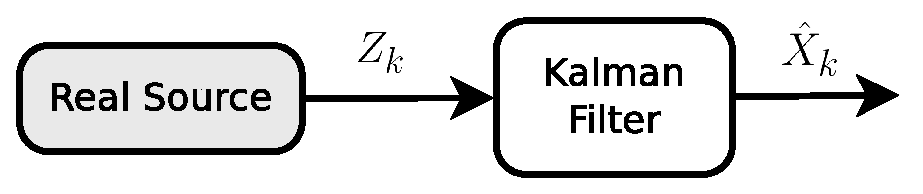
\includegraphics[width=8.0cm]{./images/KalmanModel.eps}
\caption{Modelo de filtrado Kalman em 1 dimensão.}
\label{fig:model}
\end{figure} 

O procedimento de trabalho do filtro Kalman será  explicado nas seguintes seções.


\subsection{Modelo de fonte}\label{subsec:modelfonte}
O filtro considera um modelo de fonte mais real,  onde o sinal $Z_k$
cumpre a seguinte lei de formação,
\begin{equation} \label{eq:p2}
 Z_k=H X_k +V_k.
\end{equation}
O ruido aditivo de amostras $V_k$ tem uma função de densidade de probabilidade 
do tipo Gaussiano com media zero e variância $R$, é dizer $N(0,R)$.
Assim, a fonte real $Z$ é uma versão ruidosa de uma fonte ideal $X$, que é
multiplicada por um fator $H$; este valor pode ser entendido como o ganho que tem o
sensor $Z$ ao medir um fenômeno $X$.
 A fonte real $Z$ 
tem como núcleo a fonte ideal $X$, de amostras $X_k$, que assume-se cumpre a seguinte lei de formação,
\begin{equation} \label{eq:p1}
 X_k=A X_{k-1} +U_k.
\end{equation}
Como pode-se ver, a fonte ideal $X$ é gerada de forma recursiva com um fator de crescimento $A$. 
Além disso, usa-se um alimentador de informação $U$ com amostras $U_k$, 
com uma função de densidade de probabilidade  do tipo Gaussiano 
com media zero e variância $Q$, é dizer $N(0,Q)$ \cite{caractU}.

\subsubsection{Assumindo $U$ como ruido branco}\label{subsubsection:memless}
No caso discreto, podemos chamar a um sinal como ruido branco \cite{ruidob}, quando esta representa  uma variável 
aleatória $U$ de media zero e variância finita, e tem amostras $U_k$ 
que são descorrelacionadas entre sim.
Esta característica implica que o sinal $U$ realiza transições de distintas frequências
de modo que é impossível predizer o seguinte valor  que tomará a amostra $U_k$.

Isto é particularmente interessante porque podemos interpretar a equação \eqref{eq:p1} como 
um modelo autorregressivo de ordem 1, $AR(1)$ \cite{ARp}. 
Assim, para que o modelo da equação \ref{eq:p1} seja considerado como estacionário no 
sentido amplo \cite{estaW}, a variável $A$ deve ser satisfazer a seguinte condição,
\begin{equation} \label{eq:esta1}
|A | \leq 1.
\end{equation}
Tendo em conta \eqref{eq:esta1} e um modelo $AR(1)$ para $X$, podemos ver na literatura \cite{ARp}
um conjunto de relações para $X$ :
\begin{itemize}
 \item A variância de $X$ pode ser achada se consideramos 
cada amostra $X_k$ como uma variável aleatória independente.
Assim, aplicando o operador variância, $Var(.)$, sobre a equação \eqref{eq:p1} obtemos
\begin{equation} \label{eq:AR1var}
Var(X_k)=A^2Var(X_{k-1})+Var(U_k).
\end{equation}
Cumprindo-se que
\begin{equation} \label{eq:AR1var0}
Var(X)=\frac{Q}{1-A^2}.
\end{equation}
 \item Da mesma forma, $\eta_{X}$, a media de $X$ é calculada 
 aplicado o operador esperança $E[.]$ na equação \eqref{eq:p1}, 
 \begin{equation} \label{eq:AR1var_1}
\eta_{X} \equiv E[X_k]=A E[X_{k-1}]+E[U_k],
\end{equation}
obtendo assim que $\eta_X=0$.
 \item A autocorrelação de $X$, como é expressado em \cite{ARp,art1}, cumpre a seguinte relação,
\begin{equation} \label{eq:AR1auto}
Cor(X_k,X_{k+d})=E[X_k X_{k+d}]=\frac{Q}{1-A^2} A^{|d|}. 
\end{equation}
\end{itemize}
 
Para posteriores cálculos também é importante obter a autocorrelação
da fonte $Z$, $Cor(Z_k,Z_{k+d})=E[Z_k Z_{k+d}]$. Esta expressão é obtida
conhecendo pela equação \eqref{eq:p2} que, $\eta_{Z}$, a media de $Z$ e igual a $\eta_{Z}=\eta_{X}=0$.
Agora, sabendo que a fonte $X$ e o ruido $V$ estão descorrelacionados, e que  
o ruido $V$ é uma fonte sem memória, podemos afirmar que
\begin{equation} \label{eq:AR1auto3}
Cor(Z_k,Z_{k+d})=H^2 Cor(X_k, X_{k+d})
\end{equation}   


\subsection{O algoritmo do filtro Kalman}\label{subsec:Kalman}
Este método de filtrado foi originalmente apresentado por Rudolf Kalman \cite{citeulike:347166}. 
Tem como objetivo limpar um fonte $Z$ corrompida por um ruido $V \sim N(0,R)$, 
como se viu na equação \eqref{eq:p2}. A versão filtrada de uma amostra
$Z_k$ é chamada de $\hat{X}_k$, sendo $\hat{X}_k$ uma versão aproximada de $X_k$, vista na
equação \eqref{eq:p1}.

Uma versão unidimensional do filtro de Kalman está descrita no Algoritmo \ref{algo_1}. Onde pode-se 
notar que o filtro necessita como parâmetros internos as variáveis $A$, $Q$, $H$ e $R$,
e os valores iniciais das variáveis $\hat{X}_0$ e $P_0$. O algoritmo retorna para cada valor $Z_k$ 
 um valor filtrado $\hat{X}_k$.


\begin{algorithm}[H]   \label{algo_1}
   \SetAlgoLined
   \Entrada{Sinal ruidosa  $Z_k$.}   
   \Entrada{Parâmetros do filtro $A$, $H$, $Q$ e $R$. } 

   \Saida{Sinal filtrada $\hat{X}_k$}
   \Inicio{
      Inicializa as variáveis do filtro: $\hat{X}_0=0$ e $P_0=0$. \\
      \Para{cada valor inteiro de $k$, ascendentemente }{
	  Gera uma amostra $U_k$, desde uma variável aleatória de media zero e variância $Q$.
	  \begin{equation} \label{eq:ak0}
	  U_k ~~ \sim ~~ N(0,Q).
	  \end{equation}      
	  
	  Avalia as \textbf{equações de propagação} obtendo as variáveis temporais
	  $X^-$ e $P^-$.
	  \begin{equation} \label{eq:ak1}
	  X^-=A \hat{X}_{k-1} +U_k,
	  \end{equation}
	  \begin{equation} \label{eq:ak2}
	  P^-=A P_{k-1} A + Q.
	  \end{equation}
	  
	  Calcula $K$, que é o \textbf{ganho do filtro}, 
	  \begin{equation} \label{eq:ak3}
	  K  =  P^- H/(H P^- H+R).
	  \end{equation}
	  
	  Avalia as \textbf{equações de atualização}.
	  \begin{equation} \label{eq:ak4}
	  P_k = (1-KH) P^-,
	  \end{equation}
	  \begin{equation} \label{eq:ak5}
	  \hat{X}_k=X^- + K (Z_k-H X^-).
	  \end{equation}
      }
   }
   \Retorna{$\hat{X}_k$}

   \caption{\textsc{Filtro Kalman em 1 dimensão}}
\end{algorithm}

Uma caraterística interessante do filtro é que o estado atual $\{\hat{X}_k,P_k\}$ 
só depende do estado imediato anterior  $\{\hat{X}_{k-1},P_{k-1}\}$. 
Sendo que $P_k$  é a variância dos primeiros $k$ valores de $\hat{X}$,
\begin{equation}
 P_k  = Var(\hat{X}|_{k})
\end{equation}
Ver Figura \ref{fig:filterrec}.

\begin{figure}[!ht]
\center
 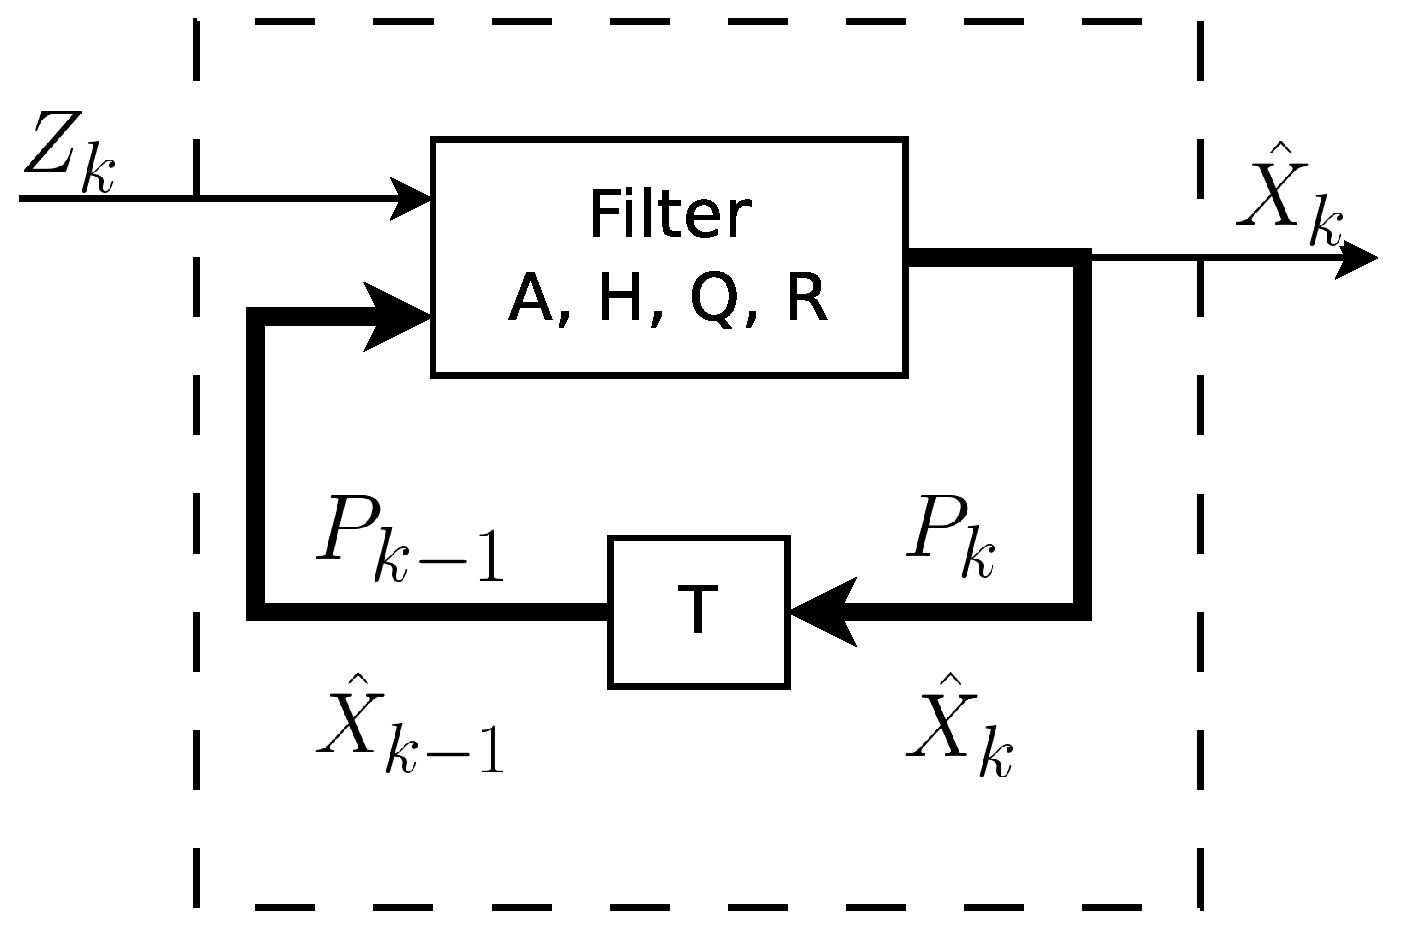
\includegraphics[width=7.0cm]{./images/KalmanFilter.eps}
\caption{Diagrama de blocos do filtro Kalman.}
\label{fig:filterrec}
\end{figure} 

\section{Cálculo de parâmetros de entrada} \label{sec:calculo}

Para poder configurar os parâmetros de entrada de um filtro Kalman de 1 dimensão,
é necessário ter os valores das variáveis $A$, $H$, $Q$ e $R$. 
Estas podem ser ordenadas em dois grupos.

Variáveis que descrevem a fonte ideal,
\begin{itemize}
 \item \textbf{A}:  Fator de crescimento da fonte ideal.
 \item \textbf{Q}:  variância do alimentador de informação da fonte ideal.
\end{itemize}
E variáveis que descrevem como o ruido é adicionado,
\begin{itemize}
 \item \textbf{H}:  Ganho de saída da fonte ideal para a fonte real.
 \item \textbf{R}:  Variança do ruido aditivo na saída real.
\end{itemize}

A escolha destes valores depende de como modelemos a fonte real $Z_k$. Como exemplo,
na seguinte seção, serão obtidas estas variáveis para o caso do filtrado da
saída de um sensor de aceleração.

\subsection{Filtrando a saída de um sensor de aceleração assumindo $H=1$} \label{sec:sensor}
O primeiro que podemos assumir, sem perda de generalidade, é que $H=1$. De modo que 
\begin{equation} \label{eq:a2}
 Z_k=X_k +V_k.
\end{equation}
Isto acontece porque dividir a $Z_k$ por um valor escalar $A$, não distorce a informação
nem afeta a fonte ideal $X_k$, só afeta linearmente ao ruido $V_k$ que ainda não foi calculado.
Agora, para obter  a variância $R$ das amostras $V_k$, $R=Var(V)$, 
podemos colocar o sensor de aceleração em repouso 
obtendo assim a saída $Z^r$ de amostras $Z^r_k$, provenientes
de uma fonte ideal em repouso $X^r$, com amostras $X^r_k=0$, de modo que $Var(X^r)=0$. 
Então, conhecendo a equação \eqref{eq:a2} 
podemos afirmar que $Var(Z^r)=Var(V)$ e consequentemente que $R=Var(Z^r)$.

Por outro lado, pelo modelo de fonte usado, soubemos que se $X$ é estacionário no sentido amplo então $|A| \leq 1$.
Mas. também é possível obter uma relação entre as variáveis $A$ e $Q$.  Para conseguir isto, com o sensor $Z$ em atividade ($Z^a$), tomaremos amostras
$Z^a_k$ de modo que se aplicamos o operador $Var()$ na equação \eqref{eq:a2} e entregamos o resultado à
equação \eqref{eq:AR1var0}, podemos afirmar que 
\begin{equation} \label{eq:a3}
 Var(X)=Var(Z^a) -  R = \frac{Q}{1-A^2}
\end{equation}
Agora, combinando as equações \eqref{eq:AR1auto}, \eqref{eq:AR1auto3}, \eqref{eq:a3}
e definindo $f_d(A)$ como uma função da variável $A$, soubemos que
\begin{equation} \label{eq:a4}
\frac{Cor(Z^a_k,Z^a_{k+d})}{Var(Z^a) -  R} = f_d(A) \equiv A^{|d|}.
\end{equation} 
Onde se usamos $d=1$ obtemos
\begin{equation} \label{eq:a5}
\frac{Cor(Z^a_k,Z^a_{k+1})}{Var(Z^a) -  R} = A.
\end{equation} 

A Tabela \ref{tab:tab1} resume o exposto anteriormente.

\begin{table}[!ht]
\centering
\caption{Definindo os parâmetros de um filtro Kalman}
\vspace{0.5cm}
\begin{tabular}{ l | p{5.0cm} | >{\centering\arraybackslash}m{3.5cm}}
\hline     
Passo & Descrição & Valor \\ % Note a separação de col. e a quebra de linhas
\hline                               % para uma linha horizontal
\hline    
1 & Assumimos o ganho de saída $H$ como unitário. & $H=1$ \\ \hline    
2 & A variância $R$ do ruido é igual à variância da saída com o sensor em repouso. & $R=Var(Z^r)$ \\ \hline    
3 & O fator de crescimento $A$ é calculado avaliando os dados $Z^a_k$, do sensor em atividade $Z^a$, na equação \eqref{eq:a5}. & $A \equiv f_1(A) = \frac{Cor(Z^a_k,Z^a_{k+1})}{Var(Z^a)-R}$ \\ \hline    
4 & Assumindo que já foi obtido um valor para $A$. $Q$ pode ser calculado com a equação \eqref{eq:a3}. & $ \frac{Q}{1-A^2}=Var(Z^a)-R$ \\ \hline     
\end{tabular}
\label{tab:tab1}
\end{table}

\subsection{Aproximando os parâmetros Kalman para valores de $R$ cercanos a $Var(X)$} \label{sec:Avalue}

A Tabela \ref{tab:tab1} mostra como obter os parâmetros do filtro Kalman quando  
se tem: um modelo de saída do sensor como na equação \eqref{eq:p2} e um modelo de fonte 
ideal como na equação \eqref{eq:p1}. Para todos os cálculos é considerado que $V$ e $U$ são fontes sem memória
de função de densidade de probabilidade Gaussiana com media nula. Na prática pode acontecer que estas
afirmações não sejam verdadeiras. Por exemplo, se a fonte $V$ for simplesmente uma
fonte ``quase sem memória'', esta teria  valores distintos de zero na sua função de autocorrelação.
Estes valores seriam desprezíveis no caso em que $R$ seja muito menor que $Var(X)$,
mas a medida que $R$ cresce a mínima autocorrelação entre os valores de $V$ pode ocasionar
que a equação \eqref{eq:a5} não seja mais verdadeira. Por este motivo o cálculo da variável $A$
como na equação \eqref{eq:a5} deve ser modificado, aceitando o fato que a equação \eqref{eq:a4}
fornece resultados ruidosos $\{\hat{f}_1, \hat{f}_2, \hat{f}_3... \}$ de uma sequencia
que deveria ser exponencialmente  decrescente como $\{A^1, A^2, A^3... \}$.
Para resolver este problema, podemos modelar o exposto anteriormente da seguinte forma.

Devemos de ter calculado os valores  ruidosos $\hat{f}_d$ usando a seguinte equação,
\begin{equation} \label{eq:a_4}
\hat{f}_d=\frac{Cor(Z^a_k,Z^a_{k+d})}{Var(Z^a) -  R}
\end{equation} 
para $d \in \{1, 2, ..., L\}$.
$L$ é um valor arbitrário a escolher, mas deve-se ter em conta que valores de $A^L$
muito pequenos tem muito ruido, então deveria de se escolher um valor de $L$
pequeno. Podemos sugerir aqui, escolher $L$ observando ate que valor de $d$ na
equação \eqref{eq:a_4}, os resultados ainda se comportam próximos a uma 
serie do tipo $\{A^1, A^2, ..., A^d, ..., A^L \}$.

Da equação \eqref{eq:a_4} obtemos um vetor coluna com os dados ruidosos, o qual chamamos de
\begin{equation} \label{eq:t0}
\hat{F}=\left(
\begin{matrix}
 \hat{f}_1\\
 \hat{f}_2\\
 \vdots\\
 \hat{f}_L\\
\end{matrix}\right).
\end{equation}
Por outro lado definimos como $F(A)$, ao vetor com os cálculos ideais $f_d(A)\equiv A^{|d|}$,
\begin{equation} \label{eq:t1}
F(A)=\left(
\begin{matrix}
 A^1\\
 A^2\\
 \vdots\\
 A^L\\
\end{matrix}\right),
\end{equation} 
e $J(A)$ como sua derivada,
\begin{equation} \label{eq:t5}
 J(A)=\frac{dF(A)}{dA}=\left(
\begin{matrix}
 1\\
 A^1\\
 A^2\\
 \vdots\\
 A^{L-1}\\
\end{matrix}\right).
\end{equation}
Assim, definiremos que o valor de $A$ desejado, é aquele valor que diminui o erro quadrático, $e^2$, em
\begin{equation} \label{eq:t3}
 e^2 = || \hat{F} - F(A) ||^2.
\end{equation}
Usando a regularização de Tikhonov \cite{shobha2014newton,doicu2002iteratively,tichonov1992ill}, para o caso não linear,
obtemos o valor de $A$ resolvendo iterativamente a seguinte 
equação,
\begin{equation} \label{eq:t4}
 A_{i+1}=A_{i}+ \left( J^T(A_{i}) J(A_{i})\right)^{-1} J^T(A_{i}) \left(\hat{F}-F(A_{i}) \right).
\end{equation}

Desta forma se aplicamos o procedimento da Tabela \ref{tab:tab1} e observamos 
que o valor da variável $R$ é próximo do valor de $Var(X)$,
então deve ser trocado o passo 3 da Tabela \ref{tab:tab1}, pela forma de cálculo
da variável  $A$ que é descrito na equação \eqref{eq:t4}.

\subsection{Se decidimos usar $H \neq 1$ } \label{sec:H}

Se temos decidido usar um valor de $H$ diferente de $1$, ainda é possível reutilizar
os cálculos explicados na Sessão \ref{sec:sensor}.
Para isto temos que considerar que na equação \eqref{eq:a2}, $H$ foi absorvido pela variável $X$,
de jeito que $X_{k}=H \bar{X}_{k}$, sendo a variável $\bar{X}$ a verdadeira fonte ideal.
Assim, aplicando esta nova relação na equação \eqref{eq:p1} obtemos
\begin{equation} \label{eq:t6}
\bar{X}_{k}=A \bar{X}_{k}+ \bar{U}_k,
\end{equation}
de jeito que a variável aleatória $\bar{U}$ terá amostras
\begin{equation} \label{eq:t7}
\bar{U}_k=\frac{U_k}{H}.
\end{equation}
Pelo qual a variância $\bar{Q}=Var(\bar{U})$ pode ser calculada como
\begin{equation} \label{eq:t8}
\bar{Q}=\frac{Q}{H^2}.
\end{equation}

Assim, podemos obter os parâmetros do filtro Kalman usando a Tabela \ref{tab:tab1},
de modo que obtemos a tupla 
\begin{equation} \label{eq:t9}
\{H=1,R,A,Q\},
\end{equation}
e se desejamos usar um valor de $H \neq 1$, transformaremos a tupla anterior em
\begin{equation} \label{eq:t10}
\{H,R,A,\frac{Q}{H^2}\}.
\end{equation}


\bibliographystyle{abbrv}
\bibliography{biblio}

\end{document}

%%%%%%%%%%%%%%%%%%%%%%%%%%%%%%%%%%%%%%%%%%%%%%%%%%%%%%%%%%%%%%%%%%%%%%%%%%%%%%%%%%%%%%%%%%%%%%%%%%%%%%%%%
%%%%%%%%%%%%%%%%%%%%%%%%%%%%%%%%%%%%%%%%%%%%%%%%%%%%%%%%%%%%%%%%%%%%%%%%%%%%%%%%%%%%%%%%%%%%%%%%%%%%%%%%%
%%%%%%%%%%%%%%%%%%%%%%%%%%%%%%%%%%%%%%%%%%%%%%%%%%%%%%%%%%%%%%%%%%%%%%%%%%%%%%%%%%%%%%%%%%%%%%%%%%%%%%%%%
%%%%%%%%%%%%%%%%%%%%%%%%%%%%%%%%%%%%%%%%%%%%%%%%%%%%%%%%%%%%%%%%%%%%%%%%%%%%%%%%%%%%%%%%%%%%%%%%%%%%%%%%%
%%%%%%%%%%%%%%%%%%%%%%%%%%%%%%%%%%%%%%%%%%%%%%%%%%%%%%%%%%%%%%%%%%%%%%%%%%%%%%%%%%%%%%%%%%%%%%%%%%%%%%%%%
%%%%%%%%%%%%%%%%%%%%%%%%%%%%%%%%%%%%%%%%%%%%%%%%%%%%%%%%%%%%%%%%%%%%%%%%%%%%%%%%%%%%%%%%%%%%%%%%%%%%%%%%%
%%%%%%%%%%%%%%%%%%%%%%%%%%%%%%%%%%%%%%%%%%%%%%%%%%%%%%%%%%%%%%%%%%%%%%%%%%%%%%%%%%%%%%%%%%%%%%%%%%%%%%%%%
%%%%%%%%%%%%%%%%%%%%%%%%%%%%%%%%%%%%%%%%%%%%%%%%%%%%%%%%%%%%%%%%%%%%%%%%%%%%%%%%%%%%%%%%%%%%%%%%%%%%%%%%%
%%%%%%%%%%%%%%%%%%%%%%%%%%%%%%%%%%%%%%%%%%%%%%%%%%%%%%%%%%%%%%%%%%%%%%%%%%%%%%%%%%%%%%%%%%%%%%%%%%%%%%%%%
%%%%%%%%%%%%%%%%%%%%%%%%%%%%%%%%%%%%%%%%%%%%%%%%%%%%%%%%%%%%%%%%%%%%%%%%%%%%%%%%%%%%%%%%%%%%%%%%%%%%%%%%%
%%%%%%%%%%%%%%%%%%%%%%%%%%%%%%%%%%%%%%%%%%%%%%%%%%%%%%%%%%%%%%%%%%%%%%%%%%%%%%%%%%%%%%%%%%%%%%%%%%%%%%%%%
%%%%%%%%%%%%%%%%%%%%%%%%%%%%%%%%%%%%%%%%%%%%%%%%%%%%%%%%%%%%%%%%%%%%%%%%%%%%%%%%%%%%%%%%%%%%%%%%%%%%%%%%%
%%%%%%%%%%%%%%%%%%%%%%%%%%%%%%%%%%%%%%%%%%%%%%%%%%%%%%%%%%%%%%%%%%%%%%%%%%%%%%%%%%%%%%%%%%%%%%%%%%%%%%%%%
%%%%%%%%%%%%%%%%%%%%%%%%%%%%%%%%%%%%%%%%%%%%%%%%%%%%%%%%%%%%%%%%%%%%%%%%%%%%%%%%%%%%%%%%%%%%%%%%%%%%%%%%%
%%%%%%%%%%%%%%%%%%%%%%%%%%%%%%%%%%%%%%%%%%%%%%%%%%%%%%%%%%%%%%%%%%%%%%%%%%%%%%%%%%%%%%%%%%%%%%%%%%%%%%%%%
%%%%%%%%%%%%%%%%%%%%%%%%%%%%%%%%%%%%%%%%%%%%%%%%%%%%%%%%%%%%%%%%%%%%%%%%%%%%%%%%%%%%%%%%%%%%%%%%%%%%%%%%%
%%%%%%%%%%%%%%%%%%%%%%%%%%%%%%%%%%%%%%%%%%%%%%%%%%%%%%%%%%%%%%%%%%%%%%%%%%%%%%%%%%%%%%%%%%%%%%%%%%%%%%%%%
%%%%%%%%%%%%%%%%%%%%%%%%%%%%%%%%%%%%%%%%%%%%%%%%%%%%%%%%%%%%%%%%%%%%%%%%%%%%%%%%%%%%%%%%%%%%%%%%%%%%%%%%%
%%%%%%%%%%%%%%%%%%%%%%%%%%%%%%%%%%%%%%%%%%%%%%%%%%%%%%%%%%%%%%%%%%%%%%%%%%%%%%%%%%%%%%%%%%%%%%%%%%%%%%%%%
%%%%%%%%%%%%%%%%%%%%%%%%%%%%%%%%%%%%%%%%%%%%%%%%%%%%%%%%%%%%%%%%%%%%%%%%%%%%%%%%%%%%%%%%%%%%%%%%%%%%%%%%%
\begin{figure}[h!]
\centering
  \begin{subfigure}[b]{0.50\textwidth}
  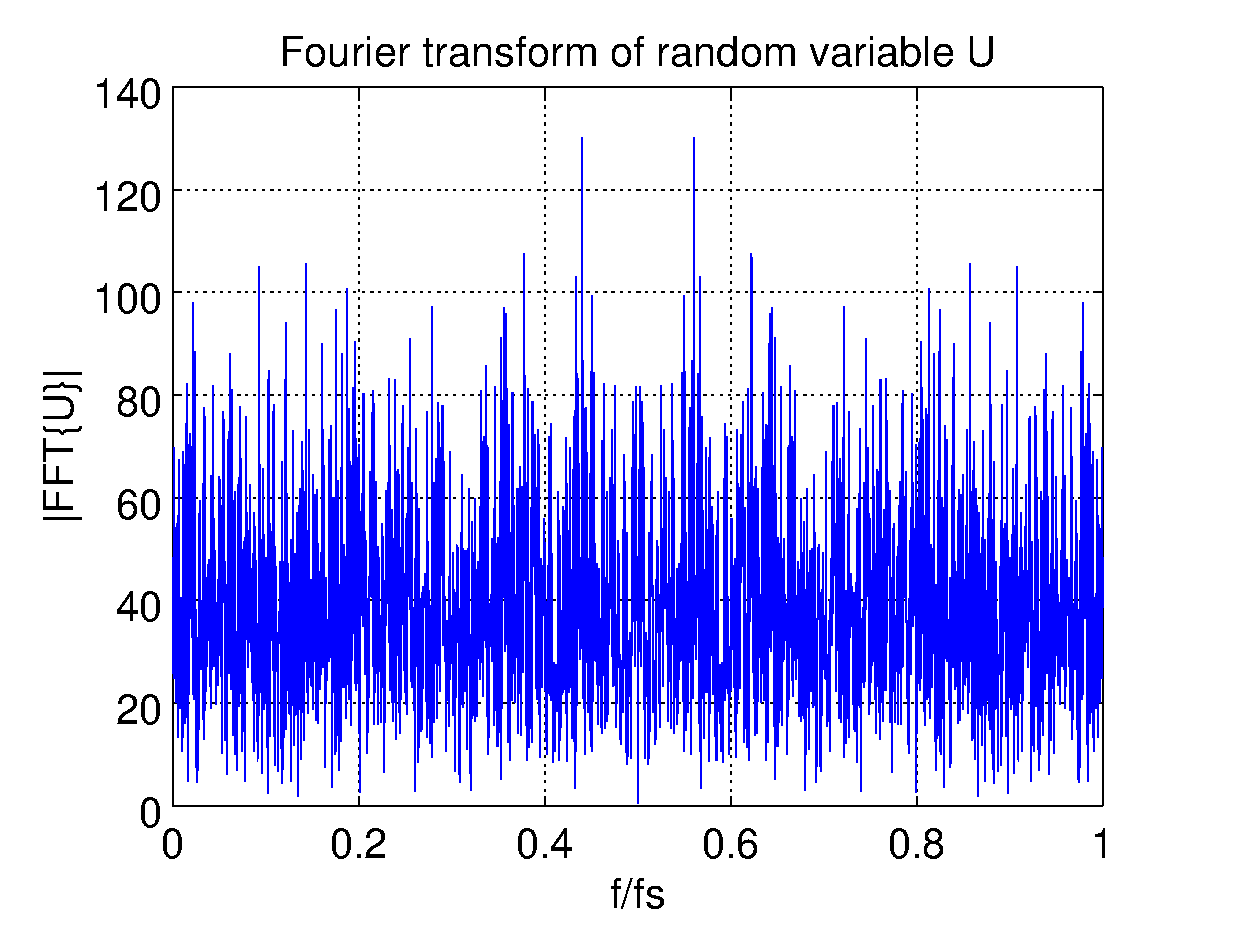
\includegraphics[width=\textwidth]{./images/fftU.eps}
  \caption{Transformada de Fourier de uma variável aleatória $U$, $N(0,1)$, com 2048 amostras.}
  \label{fig:fftU}
  \end{subfigure}
  ~
  \begin{subfigure}[b]{0.40\textwidth}
  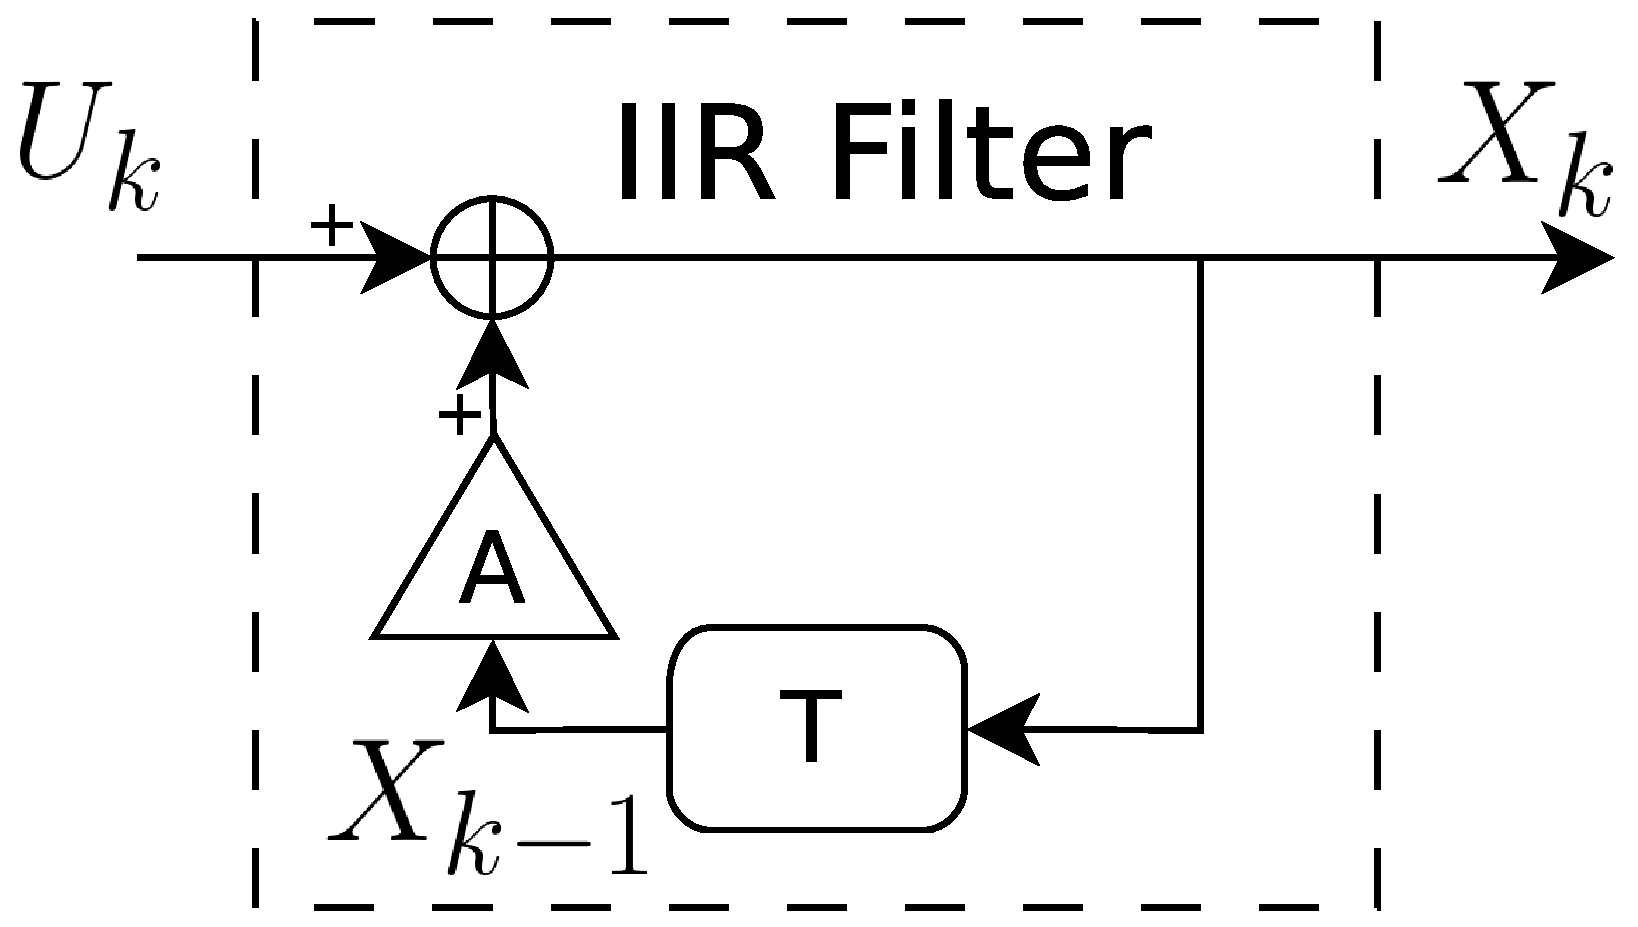
\includegraphics[width=\textwidth]{./images/filtroU.eps}
  ~\\
  \caption{Fonte $X$, interpretada como a saída de um filtro passa baixo sobre um ruido branco  $U$, $N(0,Q)$.}
  \label{fig:filtroU}
  \end{subfigure}
\caption{ Interpretando a fonte ideal $X$.} 
\label{fig:filtrofftU}
\end{figure}

Outra forma de expressar o filtro $IIR$ da equação \eqref{eq:p1} é mediante 
a seguinte equação.
\begin{equation} \label{eq:g1}
 X_{k}=\sum_{i=1}^{k}A^{k-i}U_{i}+A^k X_{0}
\end{equation}


\subsubsection{Semelhança com um filtro de resposta infinita ao impulso}
Um modelo $AR(1)$ é em essência um filtro
de resposta infinita ao impulso ($IIR$)\cite{iir}, ver Figura \ref{fig:filtroU}, 
de entrada $U_k$ e saída $X_k$, com a seguinte equação
de transferência.
\begin{equation} \label{eq:f1}
 \left |\frac{\mathbf{X}(f)}{\mathbf{U}(f)}\right |= \left |G(f)\right |=\left |\frac{1}{1-A e^{-j 2 \pi f/f_s}}\right |
\end{equation}
Onde $f_s$  é a frequência de amostragem, $f$ é a frequência em analises
e, $\mathbf{X}(f)$ e $\mathbf{U}(f)$ são as transformadas de Fourier das fontes 
$X$ e $U$ respetivamente.
Assim observando $|G(f)|$, notaremos que a equação \eqref{eq:p1}
em verdade descreve a uma fonte ideal $X$ como o resto de passar um filtro passa baixo
sobre um ruido branco $U$. A resposta do filtro cambiará dependendo do valor de $A$.
Isto pode ser observado na Figura \ref{fig:filtroiir}.
\begin{figure}[!ht]
\center
 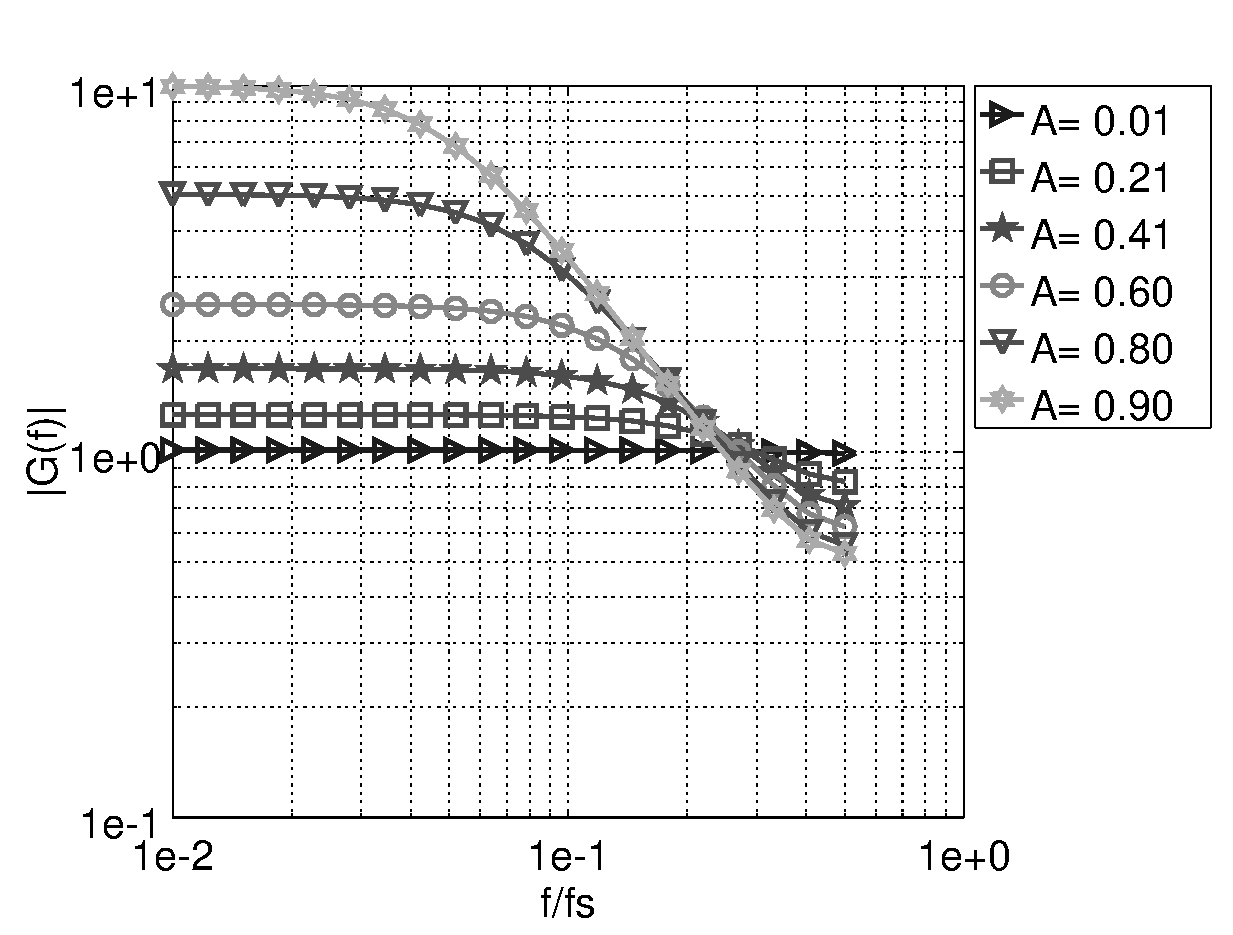
\includegraphics[width=10.0cm]{./images/filtroiir.eps}
\caption{Ganancia do filtro $IIR$ no modelo da fonte $X$.}
\label{fig:filtroiir}
\end{figure} 

Pelo qual  observaremos uma homogeneidade, para todas as frequências,  no valor absoluto da 
transformada de Fourier de $U$. Na prática, todos os valores 
girarão em torno a um valor médio como mostra a Figura \ref{fig:fftU}.


